\documentclass[a4paper,10pt]{article}
\usepackage[hidelinks]{hyperref}
\usepackage{float}
\usepackage{graphicx}
\usepackage{listings}
\usepackage[utf8]{inputenc}
\usepackage{etoolbox}
\renewcommand*\contentsname{Indice}

\makeatletter
\patchcmd\l@section{%
  \nobreak\hfil\nobreak
}{%
  \nobreak
  \leaders\hbox{%
    $\m@th \mkern \@dotsep mu\hbox{.}\mkern \@dotsep mu$%
  }%
  \hfill
  \nobreak
}{}{\errmessage{\noexpand\l@section could not be patched}}
\makeatother

\setcounter{secnumdepth}{0}

\begin{document}

\begin{titlepage}
\noindent
    \vspace*{5mm}
	\begin{minipage}[t]{0.15\textwidth}
	    \vspace*{5mm}
		\vspace{-3.5mm}{
\includegraphics{img/logo_bicocca.png}}
	\end{minipage}
	\hspace{1cm}
	\begin{minipage}[t]{0.90\textwidth}
	      \vspace*{5mm}
		{
			{\textsc{Università degli Studi di Milano - Bicocca} } \\
			\textbf{Scuola di Scienze} \\
			\textbf{Dipartimento di Informatica, Sistemistica e Comunicazione} \\
			\textbf{Corso di Laurea Magistrale in Informatica} \\
			\par
		}
	\end{minipage}
	
	\vspace{42mm}

\begin{center}
    {\LARGE{
    
            \textbf{Metodi del Calcolo Scientifico - Progetto 1 \\ Algebra lineare numerica \\ Sistemi lineari con matrici sparse simmetriche e definite positive}
    }}        
\end{center}

\vspace{40mm}
	
	
	\begin{flushright}
		\large{Alberici Federico - 808058\\} 
		\large{Bettini Ivo Junior - 806878\\} 
		\large{Cocca Umberto - 807191\\} 
		\large{Traversa Silvia - 816435} 
	\end{flushright}
	
	\vspace{15mm}
	\begin{center}
		{\large{\bf Anno Accademico 2019 - 2020}}
	\end{center}


\end{titlepage}

\tableofcontents

\newpage

\section{Introduzione}

Lo scopo di questo progetto è studiare l’implementazione del metodo di Cholesky per la risoluzione di sistemi lineari con matrici sparse, simmetriche e definite positive, in ambienti di programmazione open source e confrontarla con l’implementazione MATLAB. Questo confronto viene eseguito su due sistemi operativi diversi, Windows e Linux.

Per ognuna delle matrici calcoliamo:
\begin{itemize}
\item Il tempo necessario per calcolare la soluzione x del sistema lineare Ax=b
\item L’errore relativo tra la soluzione calcolata x e la soluzione esatta xe, trovata come soluzione del sistema Axe=B
\item La memoria necessaria per risolvere il sistema, ovvero l’aumento della dimensione del programma in memoria da subito dopo aver letto la matrice a dopo aver risolto il sistema.
\end{itemize}

Per poter raggiungere questo obiettivo abbiamo deciso di confrontare MATLAB con gli ambienti open source C++, R e Python.
È possibile trovare il listato dei codici alla seguente \href{https://gitlab.com/okamiRvS/cholesky-computing}{repository}

\newpage

\section{MATLAB}

MATLAB è un ambiente per il calcolo numerico e l’analisi statistica scritto in C. 
Nella scrittura del codice, per prima cosa abbiamo importato le diverse matrici attraverso la funzione mmread nel formato .mtx  (invece del formato MATLAB .mat) in modo da mantenere linearità con gli altri linguaggi usati.


\begin{figure}[H]
\centering
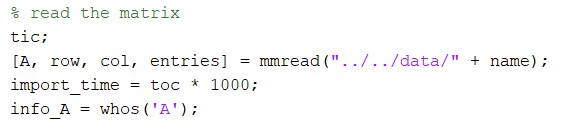
\includegraphics[width=0.6\linewidth]{img/matlab1.jpg}
%\caption{\textit{}}
\label{fig:1}
\end{figure}

Attraverso la funzione tic toc abbiamo calcolato il tempo di esecuzione specifiche porzioni del codice di interesse, come il calcolo della decomposizione di Cholesky e della soluzione finale del sistema lineare.
Dopo aver calcolato la soluzione esatta xe del sistema lineare A*xe = b, attraverso il comando Chol abbiamo eseguito la decomposizione di Cholesky. 

\begin{figure}[H]
\centering
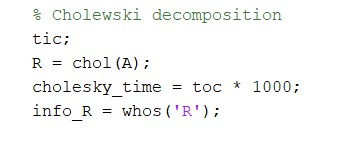
\includegraphics[width=0.45\linewidth]{img/matlab2.jpg}
%\caption{\textit{}}
\label{fig:2}
\end{figure}

La funzione chol è in grado di accorgersi se la matrice passata è definita positiva e simmetrica. Dopo aver determinato lo spazio in memoria occupato dalla matrice decomposta attraverso il metodo di Cholesky abbiamo calcolato la soluzione finale x, grazie alla quale abbiamo potuto trovare l’errore relativo e abbiamo infine misurato il tempo di risoluzione.

Abbiamo gestito eventuali eccezioni generate durante l’esecuzione del programma attraverso un catch exception, che ci ha permesso di accorgerci che MATLAB va in “out of memory” con matrici particolarmente grandi (con matrici di dimensione superiore a cfd2.mtx, la quale ha 123,440 righe e colonne).

\newpage 

\section{C++}

La decomposizione di Cholesky è stata effettuata sfruttando Eigen, libreria template per l’algebra lineare. Delle numerose funzionalità messe a disposizione sono stati usati i moduli Sparse per la gestione di matrici sparse e SparseCholesky per la decomposizione.

Il programma è compilabile tramite Makefile presente nella cartella dei sorgenti (./src/c++/) e va eseguito via riga di comando fornendo come parametro la cartella in cui sono inserite le matrici in formato Matrix Market (es. \$./main.out ../../data)
L’analisi viene eseguita su tutte le matrici .mtx presenti nella cartella data.

Il primo problema affrontato è stata l’importazione in memoria del formato .mtx. Nonostante esistano delle funzioni di import reperibili online ( \href{https://math.nist.gov/MatrixMarket/mmio-c.html}{MatrixMarket/mmio-c.html}) abbiamo deciso di scrivere un parser ad-hoc per matrici Matrix Market.

\begin{figure}[H]
\centering
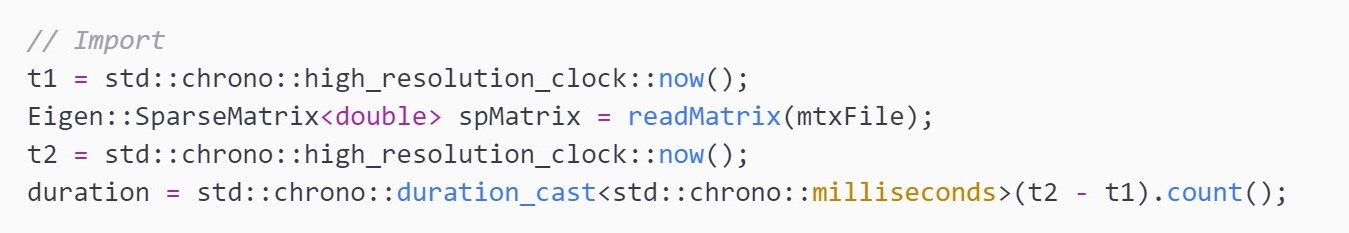
\includegraphics[width=0.7\linewidth]{img/c++1.jpg}
\caption{\textit{Import tramite funzione custom Eigen::SparseMatrix<double> readMatrix(std::string \&filename)}}
%\label{fig:1}
\end{figure}

Non avendo trovato una funzione che permettesse di controllare lo spazio in memoria occupato da un oggetto, la dimensione delle matrici è stata calcolata empiricamente, studiandone la metodologia di memorizzazione. 
Eigen (così come la libreria utilizzata per il linguaggio Python) comprime la matrice sparsa utilizzando il formato Compressed Sparse Row/Column. Vengono mantenuti in memoria due array di interi (4 byte), contenti indici per la ricostruzione della matrice, e un array di double (8 byte), contenete i valori non-zero.

\begin{figure}[H]
\centering
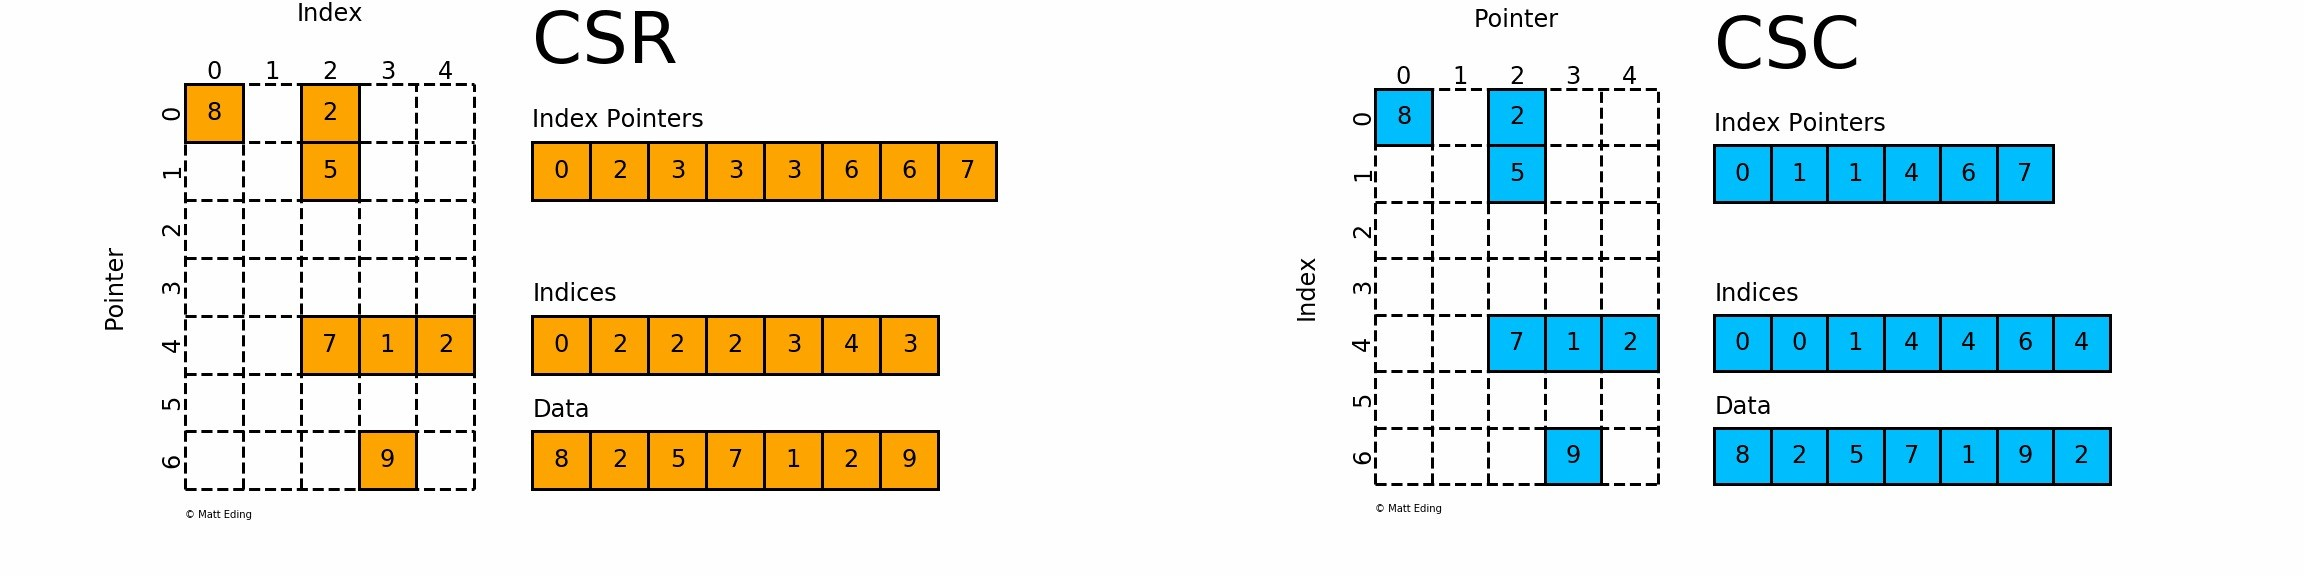
\includegraphics[width=0.7\linewidth]{img/c++2.jpg}
\caption{\textit{formato CSR e CSC}}
%\label{fig:1}
\end{figure}

Il calcolo per ricavare la dimensione della matrice è quindi il seguente: \\
\textit{MatrixSize = (Inner\_Pointers.size() + Indices.size()) * 4 + (Data.size() * 8) [byte]} \\

A fronte di ulteriori strutture interne della libreria tale metodo permette di ottenere una buona approssimazione del costo in termini di memoria.

I passi dell’analisi sono gli stessi eseguiti in MATLAB, utilizzando opportunamente la sintassi C++ e la libreria Eigen.\\
In particolare la decomposizione di Cholesky viene calcolata tramite la funzione Eigen::SimplicialLLT<Eigen::SparseMatrix<double>> chol che riduce il fill-in applicando una permutazione simmetrica prima della fattorizzazione. %da sistemare

\newpage

\section{R}

R è un linguaggio di programmazione e ambiente di sviluppo opensource disponibile per diversi sistemi operativi, tra i quali Linux e Windows.
Inizialmente il codice è stato scritto sfruttando la libreria Matrix, ma abbiamo riscontrato che essa non permette la lettura di matrici di dimensioni elevate, abbiamo deciso dunque di ricorrere alla libreria spam. Come riporta la documentazione ufficiale infatti questa libreria è veloce e scalabile, con il pacchetto di estensione spam64 che abbiamo usato.
Importiamo la matrice con la funzione read.MM, che ci permette di salvarla in formato sparso.
Grazie al comando chol.spam effettuiamo la decomposizione di Cholesky sulla matrice in esame. Essa deve essere simmetrica e definita positiva: queste due caratteristiche vengono verificate automaticamente dalla funzione stessa, che restituisce un errore nel caso in cui queste non siano rispettate, motivo per il quale è stato inserito un blocco try-catch.

\begin{figure}[H]
\centering
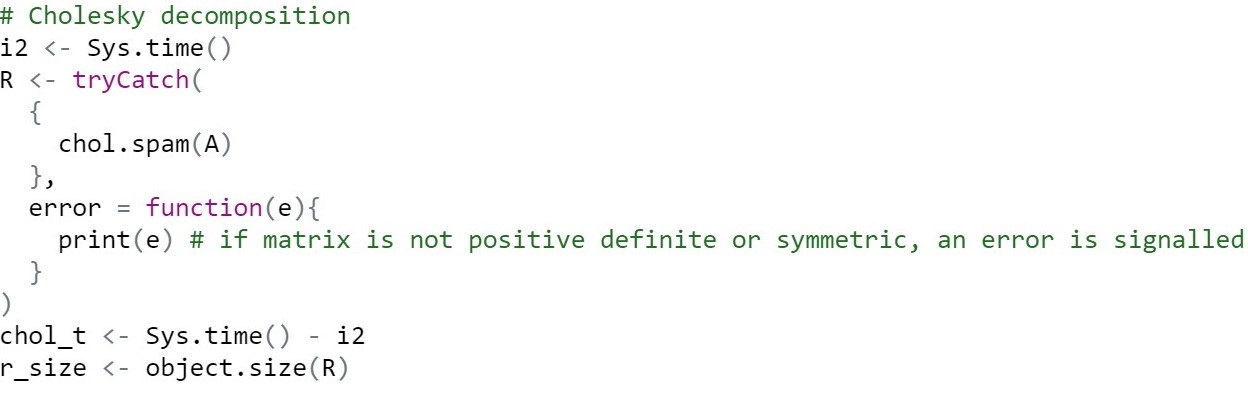
\includegraphics[width=0.8\linewidth]{img/R1.jpg}
%\caption{\textit{formato CSR e CSC}}
%\label{fig:1}
\end{figure}

La libreria in uso implementa anche la funzione solve.spam che, dato in input il risultato della funzione chol.spam, calcola direttamente il risultato del sistema lineare, combinando in maniera opportuna backsolve e forwardsolve. 

Come in MATLAB e negli altri linguaggi di programmazione considerati, abbiamo calcolato l’utilizzo della memoria, il tempo necessario per la risoluzione del sistema lineare e l’errore relativo. 

\newpage

\section{Python}

In python, il calcolo della decomposizione di Cholesky può essere eseguito con la libreria numpy e scipy per matrici dense e con scikits.sparse per le matrici sparse. Il pacchetto scikit-sparse espande scipy.sparse ritornando le matrici in formato CSC . 

Seppur il pacchetto scikits.sparse a detta dei creatori è usabile sia in ambiente Windows che Linux, in realtà ci sono dei problemi di installazione lato windows, come si può vedere nella schermata issues della repository ufficiale. Per installare il pacchetto su Windows infatti è stato necessario come prima cosa compilare attraverso cmake suite sparse, una libreria C/C++ che permette di eseguire operazioni su matrici sparse. Così facendo siamo in grado di generare le librerie della suite attraverso la build in release mode su Visual Studio. Una volta ottenuta la libreria abbiamo installato manualmente scikits.sparse per windows. 

Le operazioni base eseguite dal programma sono le medesime effettuate negli altri linguaggi considerati. In particolare, la memoria occupata è stata calcolata empiricamente come visto in C++ poiché anche scikit sparse salva in memoria le matrici nello stesso formato di Eigen. Il calcolo della decomposizione di Cholesky, poi, è stato eseguito con la funzione cholesky(), la quale ritorna un risolutore factor. Quest’ultimo permette di risolvere il sistema lineare Ax = b come mostrato nella figura:

\begin{figure}[H]
\centering
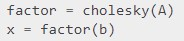
\includegraphics[width=0.4\linewidth]{img/python1.jpg}
%\caption{\textit{formato CSR e CSC}}
%\label{fig:1}
\end{figure}

\newpage

\section{Analisi dei risultati}
Per l’analisi confrontiamo i grafici derivanti dai risultati ottenuti in output dalle varie esecuzioni dei linguaggi nei due sistemi operativi Linux e Windows. 
La raccolta dei dati è avvenuta su un unico pc provvisto di macchina virtuale per entrambi i sistemi operativi, in modo tale da avere una potenza di calcolo confrontabile statisticamente.
Le specifiche tecniche sono le seguenti: \\

\textbf{Windows x64} 
\textit{Processor: Intel(R) Core(TM) i5-4460  CPU @ 3.20GHz, Number of cores: 4, Memory: Ram 11000 MB\\}

\textbf{Unix x64} 
\textit{Kernel: 5.3.0-53-generic, Processor: Intel(R) Core(TM) i5-4460  CPU @ 3.20GHz, Number of cores: 4, Memory: Ram 11000 MB\\}


I grafici scelti sono a linee con indicatori, dove sulle ascisse troviamo le matrici in ordine crescente per dimensione e sulle ordinate le tre grandezze richieste dal progetto:
\begin{itemize}
\item chol\_size = memoria occupata dalla matrice decomposta con il metodo di Cholesky;
\item total\_time = somma del tempo necessario per la decomposizione di Cholesky e del tempo necessario per la risoluzione del sistema lineare data la matrice decomposta;
\item err = errore relativo.
\end{itemize}
Nelle ordinate viene utilizzata una scala logaritmica poiché si hanno tre valori con ordini di grandezza diversi.
 

\subsection{MATLAB}


\begin{figure}[H]
\centering
\begin{minipage}{.6\textwidth}
  \centering
  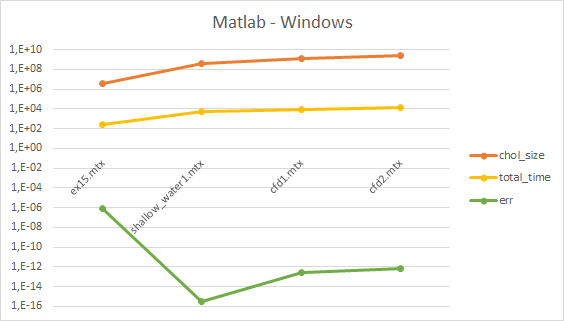
\includegraphics[width=1\linewidth]{img/matlabwin.png}
\end{minipage}%
\begin{minipage}{.6\textwidth}
  \centering
  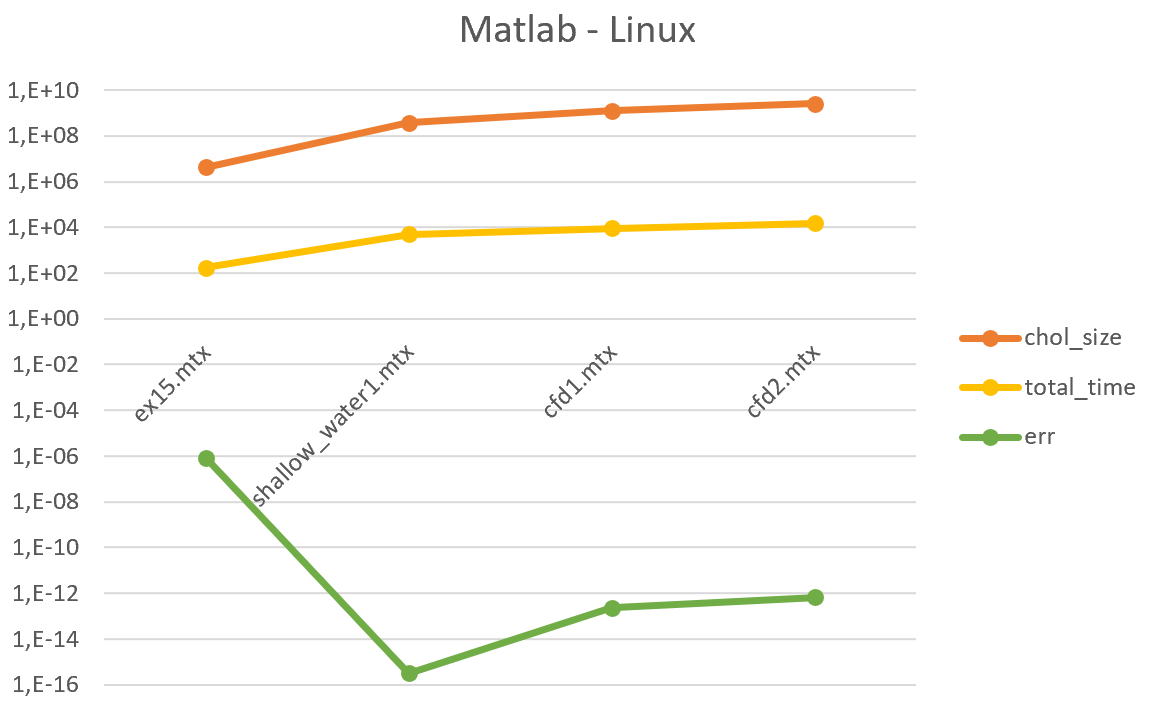
\includegraphics[width=1\linewidth]{img/matlablinux.png}
\end{minipage}
\end{figure}


In entrambi i casi al crescere della dimensione della matrice aumenta il tempo di esecuzione e la memoria da queste occupata e si ha un andamento simile per l’errore relativo. È interessante evidenziare il picco verso il basso che si ottiene con la matrice shallow\_water1, per la quale si ha l’errore relativo minore (ordine di grandezza 10-16)

Con MATLAB non è stato possibile analizzare matrici di dimensioni superiori a cfd2, in quanto il programma ci ritorna un errore out of memory. 

\subsection{C++}

\begin{figure}[H]
\centering
\begin{minipage}{.6\textwidth}
  \centering
  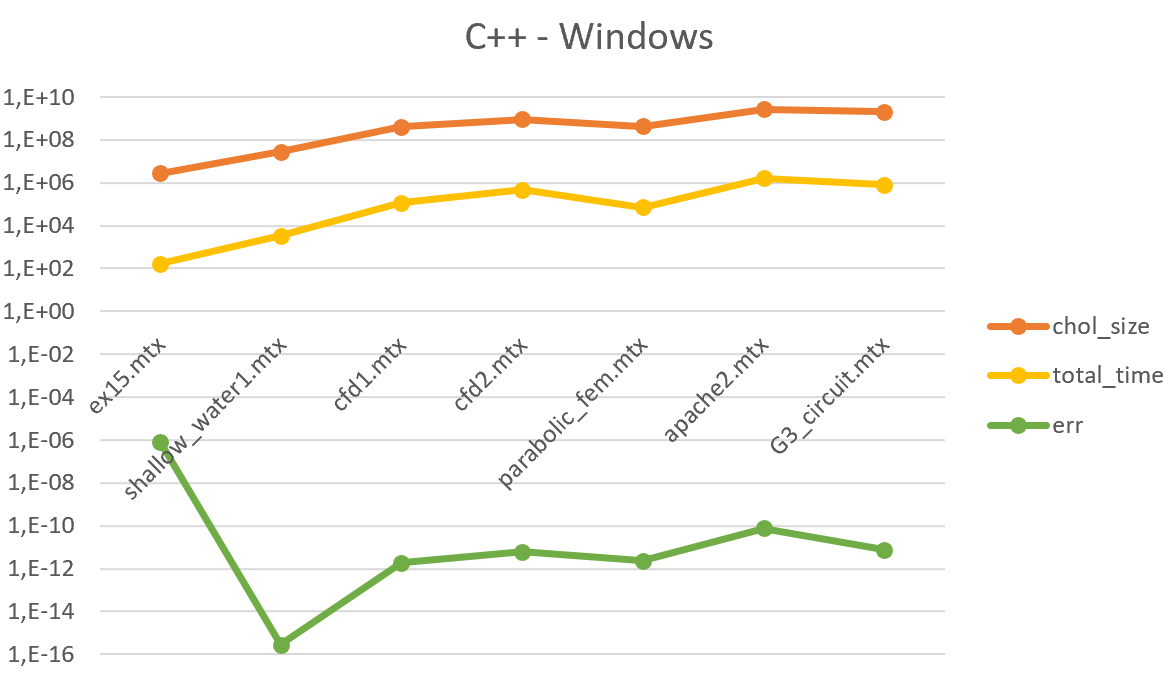
\includegraphics[width=1\linewidth]{img/c++win.png}
\end{minipage}%
\begin{minipage}{.6\textwidth}
  \centering
  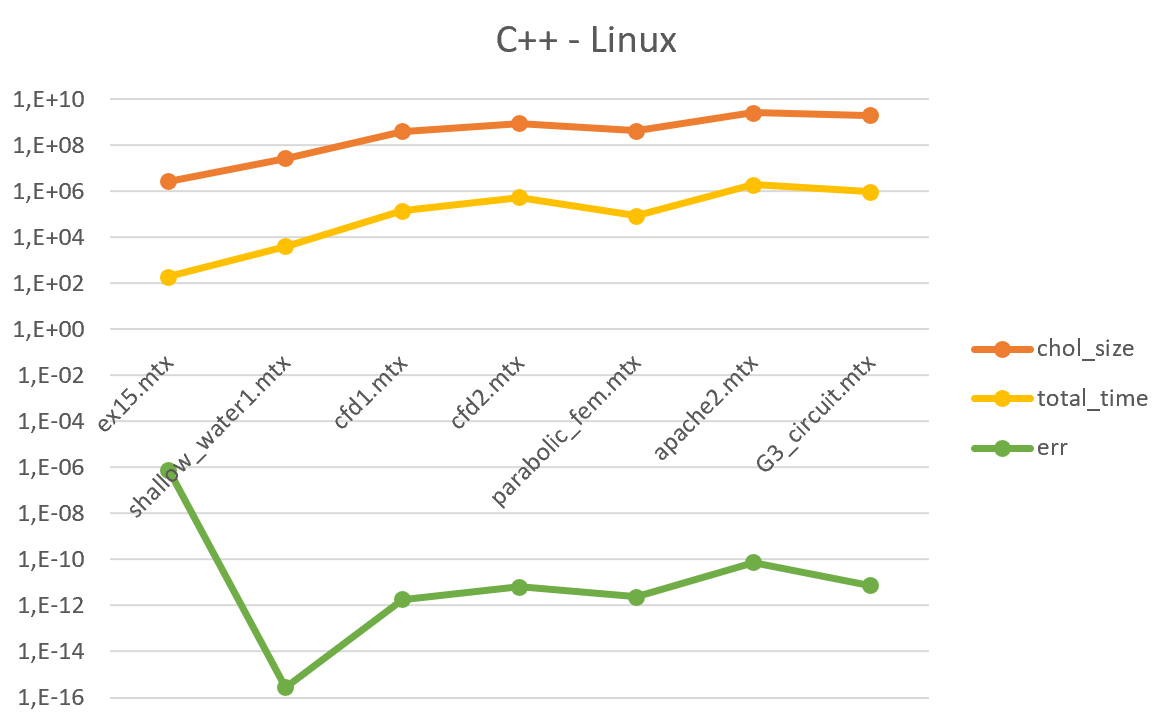
\includegraphics[width=1\linewidth]{img/c++linux.png}
\end{minipage}
\end{figure}

Anche nel caso di C++ analizzando i grafici si possono notare andamenti simili.
In Windows abbiamo una situazione abbastanza lineare per quanto riguarda la memoria occupata e il tempo, con una crescita dei due valori con l’aumentare della dimensione delle matrici, eccezione fatta per una lieve flessione con la matrice parabolic\_fem. 
Lo stesso scenario è possibile osservarlo nel grafico riferito al sistema operativo Linux.
In entrambi i casi l’errore relativo ha valori altalenanti, è interessante sottolineare che per entrambi i sistemi operativi si ha un picco verso il basso con la matrice shallow\_water1 (errore con ordine di grandezza 10-16) mentre con la matrice ex15 si ha un errore relativamente alto rispetto alle altre matrici (ordine di grandezza 10-6).

\subsection{R}


\begin{figure}[H]
\centering
\begin{minipage}{.6\textwidth}
  \centering
  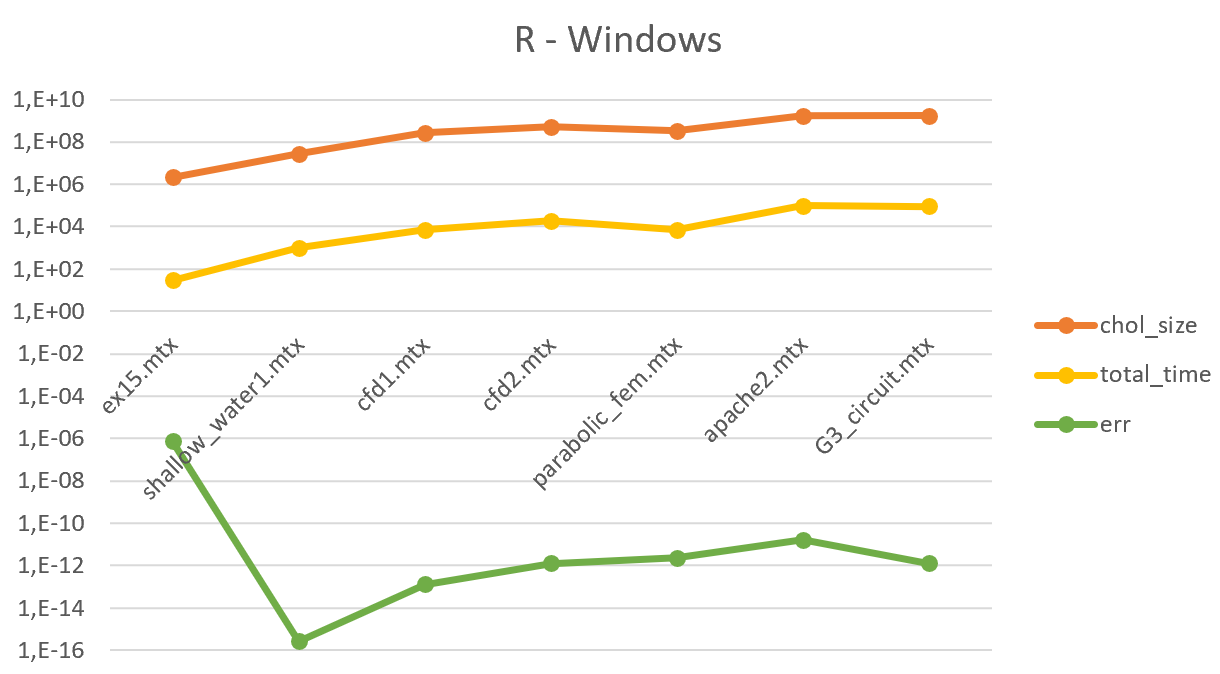
\includegraphics[width=1\linewidth]{img/Rwin.png}
\end{minipage}%
\begin{minipage}{.6\textwidth}
  \centering
  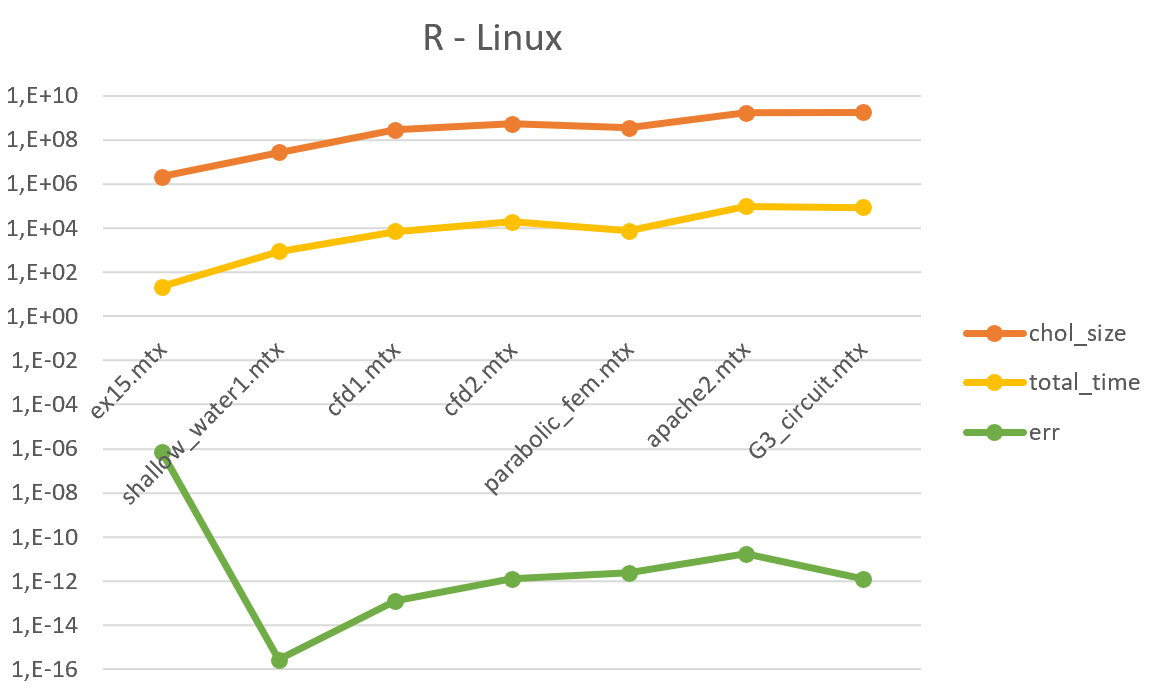
\includegraphics[width=1\linewidth]{img/Rlinux.png}
\end{minipage}
\end{figure}


In entrambi i casi al crescere della matrice cresce il tempo necessario per calcolare la soluzione finale e la memoria occupata, tranne che per una lieve flessione che si ottiene con la matrice parabolic\_fem. 
Per quanto riguarda gli errori relativi si parte in entrambe i casi con un errore relativamente alto (ordine di grandezza 10-6) per la matrice ex15, si ha poi un picco verso il basso con la matrice shallow\_water1 (raggiungendo l’ordine di grandezza 10-16), mentre procedendo con matrici più grandi aumenta lievemente l’errore, tranne nel caso di G3\_circuit dove si ha una lieve flessione. 


\subsection{Python}

\begin{figure}[H]
\centering
\begin{minipage}{.6\textwidth}
  \centering
  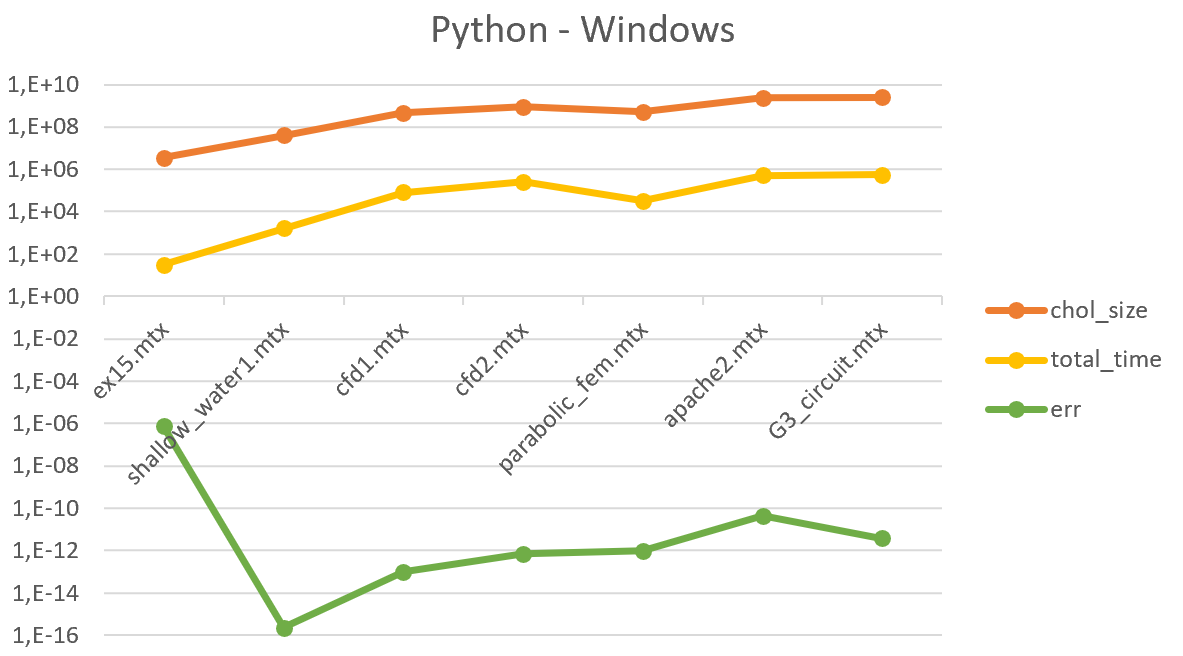
\includegraphics[width=1\linewidth]{img/pythonwin.png}
\end{minipage}%
\begin{minipage}{.6\textwidth}
  \centering
  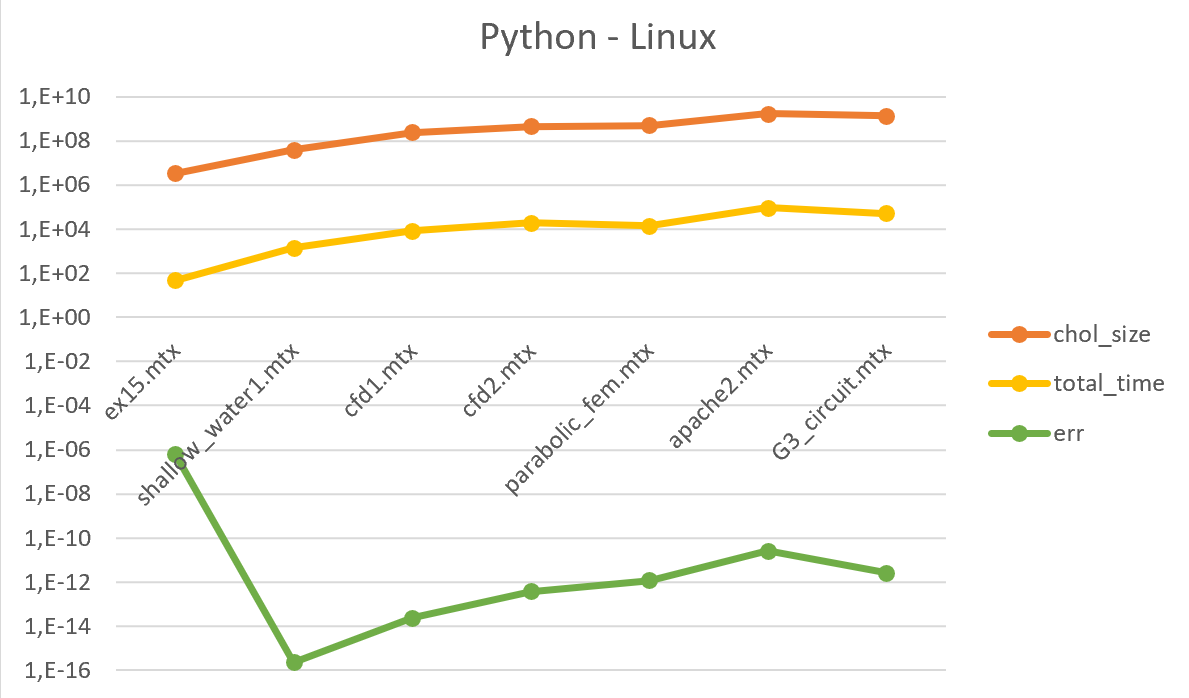
\includegraphics[width=1\linewidth]{img/pythonlinux.png}
\end{minipage}
\end{figure}


Al crescere della dimensione delle matrici aumenta la memoria occupata e il tempo di risoluzione, con una lieve flessione nel caso della matrice parabolic\_fem.
L’errore relativo ha un massimo con la matrice più piccola (ex15), raggiunge poi un minimo con la matrice shallow\_water1 ed infine tende lievemente a crescere con l’aumentare della dimensione della matrice, con una flessione finale per la matrice G3\_circuit.

\newpage

\section{Conclusioni}

Alla luce di quanto abbiamo appena analizzato e mettendoci nell’ottica proposta all’inizio del progetto, ossia immaginare di dover scegliere per un’azienda un ambiente di programmazione in grado di risolvere con il metodo di Cholesky sistemi lineari con matrici sparse e definite positive di grandi dimensioni, dovendo decidere tra software proprietario (MATLAB) oppure open source e anche tra sistema operativo Windows oppure Linux, possiamo concludere quanto segue.\\

Come prima cosa è risultato evidente che per eseguire tutte le matrici proposte è necessario disporre di computer molto potenti, indipendentemente dal sistema operativo: non è stato possibile infatti eseguire i codici con le matrici Flan 1565 e StocF-1465, rispettivamente di dimensioni 1,564,794 x 1,564,794 e 1,465,137 x 1,465,137.\\

Nel sistema operativo Windows nessuno dei linguaggi analizzati dimostra di riuscire ad eseguire i calcoli in un tempo totale (calcolato come somma del tempo necessario per l'importazione della matrice e del tempo necessario per la decomposizione di Cholesky) particolarmente migliore rispetto agli altri.

\begin{figure}[H]
\centering
  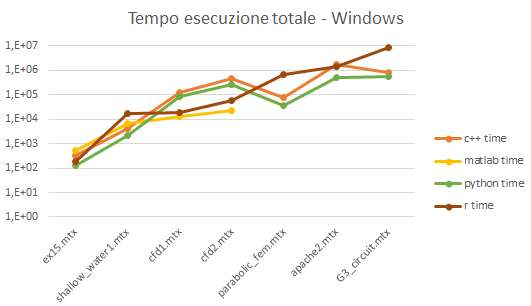
\includegraphics[width=0.6\linewidth]{img/tempototwin.png}
\end{figure}

Per quanto riguarda Linux, invece, C++ ha dei risultati decisamente peggiori mentre R risulta avere dei tempi migliori per tutte le matrici esclusa G3\_circuit, la matrice di dimensione maggiore, dove è Python ad ottenere il risultato più basso.

\begin{figure}[H]
\centering
  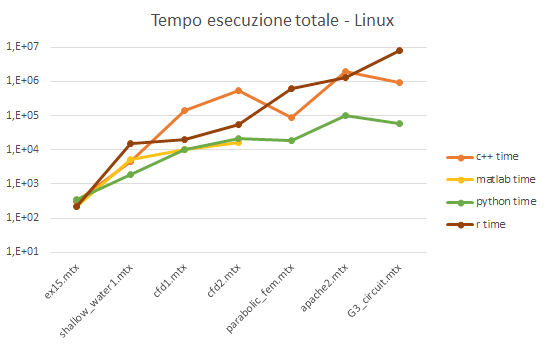
\includegraphics[width=0.6\linewidth]{img/tempototlinux.png}
\end{figure}

Esaminando però separatamente il tempo di import e il tempo della decomposizione di Cholesky, si può notare che su Windows R impiega molto più tempo per importare le matrici mentre è Python il più veloce.

\begin{figure}[H]
\centering
  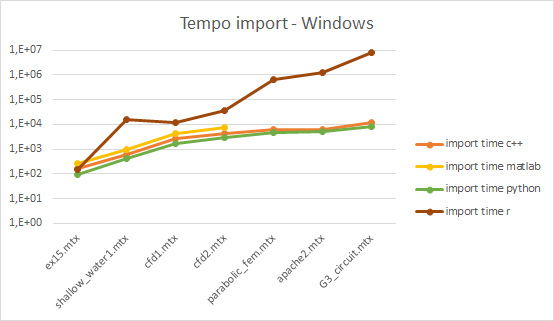
\includegraphics[width=0.6\linewidth]{img/tempoimpwin.png}
\end{figure}

Anche su Linux è R ad avere il peggior tempo di import, mentre in questo caso è MATLAB il più veloce.
\begin{figure}[H]
\centering
  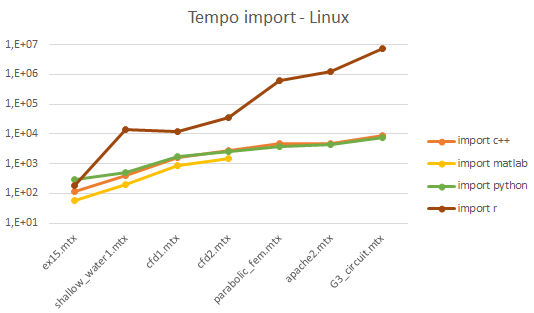
\includegraphics[width=0.57\linewidth]{img/tempoimplinux.png}
\end{figure}


MATLAB è, invece, il più lento per quanto riguarda la decomposizione di Cholesky su Windows, mentre R in questo caso è il più veloce.

\begin{figure}[H]
\centering
  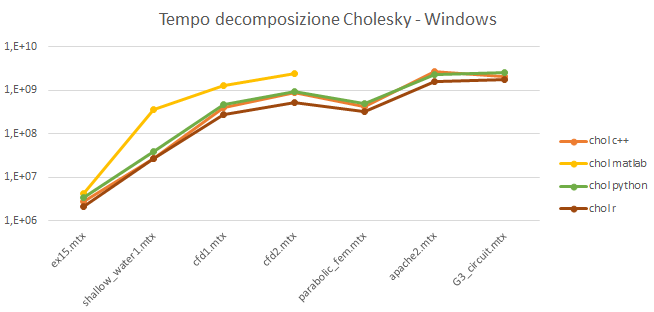
\includegraphics[width=0.6\linewidth]{img/tempocholwin.png}
\end{figure}

Su Linux, R e Python hanno i tempi peggiori, con valori molto simili, e il più veloce in questo caso è MATLAB. Se si considera, però, il fatto che con MATLAB non si riescono ad analizzare le matrici di dimensione più elevate, è C++ il linguaggio con i risultati migliori.
\begin{figure}[H]
\centering
  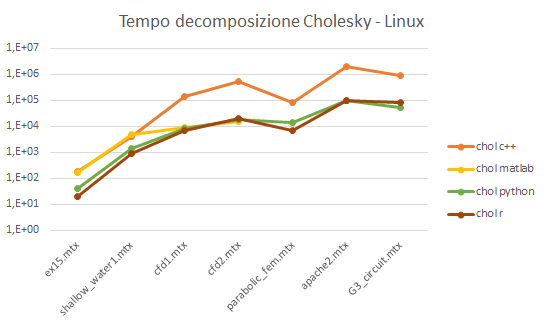
\includegraphics[width=0.6\linewidth]{img/tempochollinux.png}
\end{figure}


Per quanto riguarda l'accuratezza, in Windows R e MATLAB hanno errori di ordine di grandezza simile, con Python si ottiene un errore nettamente migliore per quanto riguarda la matrice ex\_15. Con il crescere della dimensione della matrice nessuno dei linguaggi ottiene dei risultati migliori, in quanto sono tutti altalenanti ma con ordini di grandezza simili.

\begin{figure}[H]
\centering
  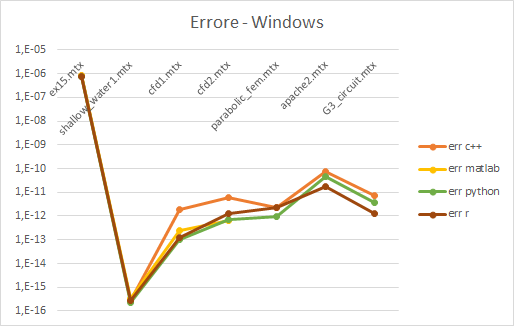
\includegraphics[width=0.5\linewidth]{img/errwin.png}
\end{figure}

In Linux, invece, si può notare che con Python si hanno errori di ordine di grandezza minore rispetto agli altri, mentre C++ ha una accuratezza minore.
 
\begin{figure}[H]
\centering
  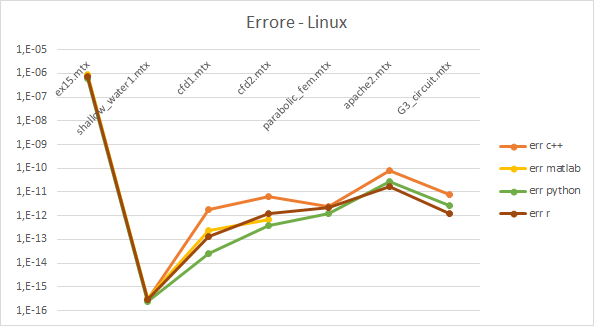
\includegraphics[width=0.5\linewidth]{img/errlinux.png}
\end{figure}

Per valutare la memoria occupata dal programma abbiamo sommato la dimensione della matrice importata e la dimensione della decomposizione di Cholesky. MATLAB è il linguaggio di programmazione che, in Windows, occupa più memoria, mentre Python, R e C++ hanno un andamento analogo, con risultati lievemente migliori per R.

\begin{figure}[H]
\centering
  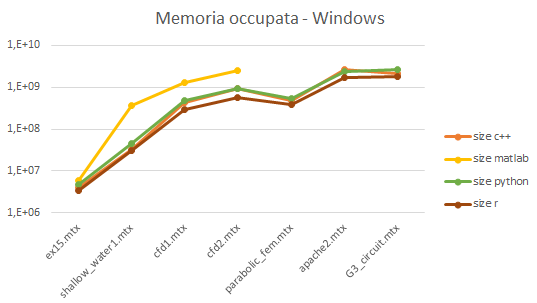
\includegraphics[width=0.5\linewidth]{img/memoccwin.png}
\end{figure}

Anche su Linux la situazione è analoga, con MATLAB ad occupare più memoria e Python, R e C++ con andamento simile.

\begin{figure}[H]
\centering
  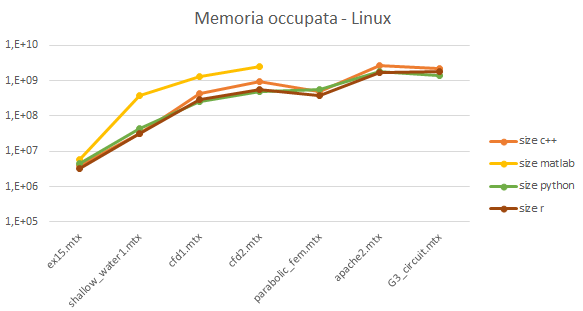
\includegraphics[width=0.5\linewidth]{img/memocclinux.png}
\end{figure}


Per quanto concerne la facilità d'uso Python è stato il linguaggio che ha causato più difficoltà nell'installazione, sopratutto su sistema operativo Windows, a causa anche dalla poca documentazione reperibile, anche se nella scrittura del codice non si incontrano particolari difficoltà. In C++ è stata utilizzata la libreria Eigen, la quale è molto ben documentata e semplice da importare ed utilizzare nel proprio programma.
I codici in MATLAB ed R sono i più immediati da scrivere, poiché nel primo caso non è necessario effettuare alcuna ricerca di librerie esterne, mentre nel caso di R si ha una documentazione ricca che permette di sfruttare al meglio le librerie disponibili.


\end{document}